\documentclass[algorithm,pgfplots]{cuzbeamer}
\usefonttheme{serif}
\setCJKmainfont{Noto Sans CJK SC}
\usepackage[scale=2]{ccicons}

\begin{document}
    \title{基于 Spark 的 pagerank 算法实现与原理解析}
\date{\today}
\author{刘佳玮,计算机科学与技术学院,20031211496, 刘佳玮,计算机科学与技术学院,20031211496}
\email{https://github.com/muyuuuu/Spark-learn}
    \maketitle

    \begin{frame}{大纲}
        \setbeamertemplate{section in toc}[sections numbered]
        \tableofcontents
    \end{frame}

    \section{好的算法与好的设备}

    \begin{frame}{算法时间复杂度}
        \begin{leftbar}
            同一个问题,一个时间复杂度$O(n^2)$与$O(n^3)$的时间对比,代码开放于:
            {\sffamily \url{https://github.com/muyuuuu/Algorithm/tree/master/Insert_sort}}
        \end{leftbar}
        \begin{figure}[h]
            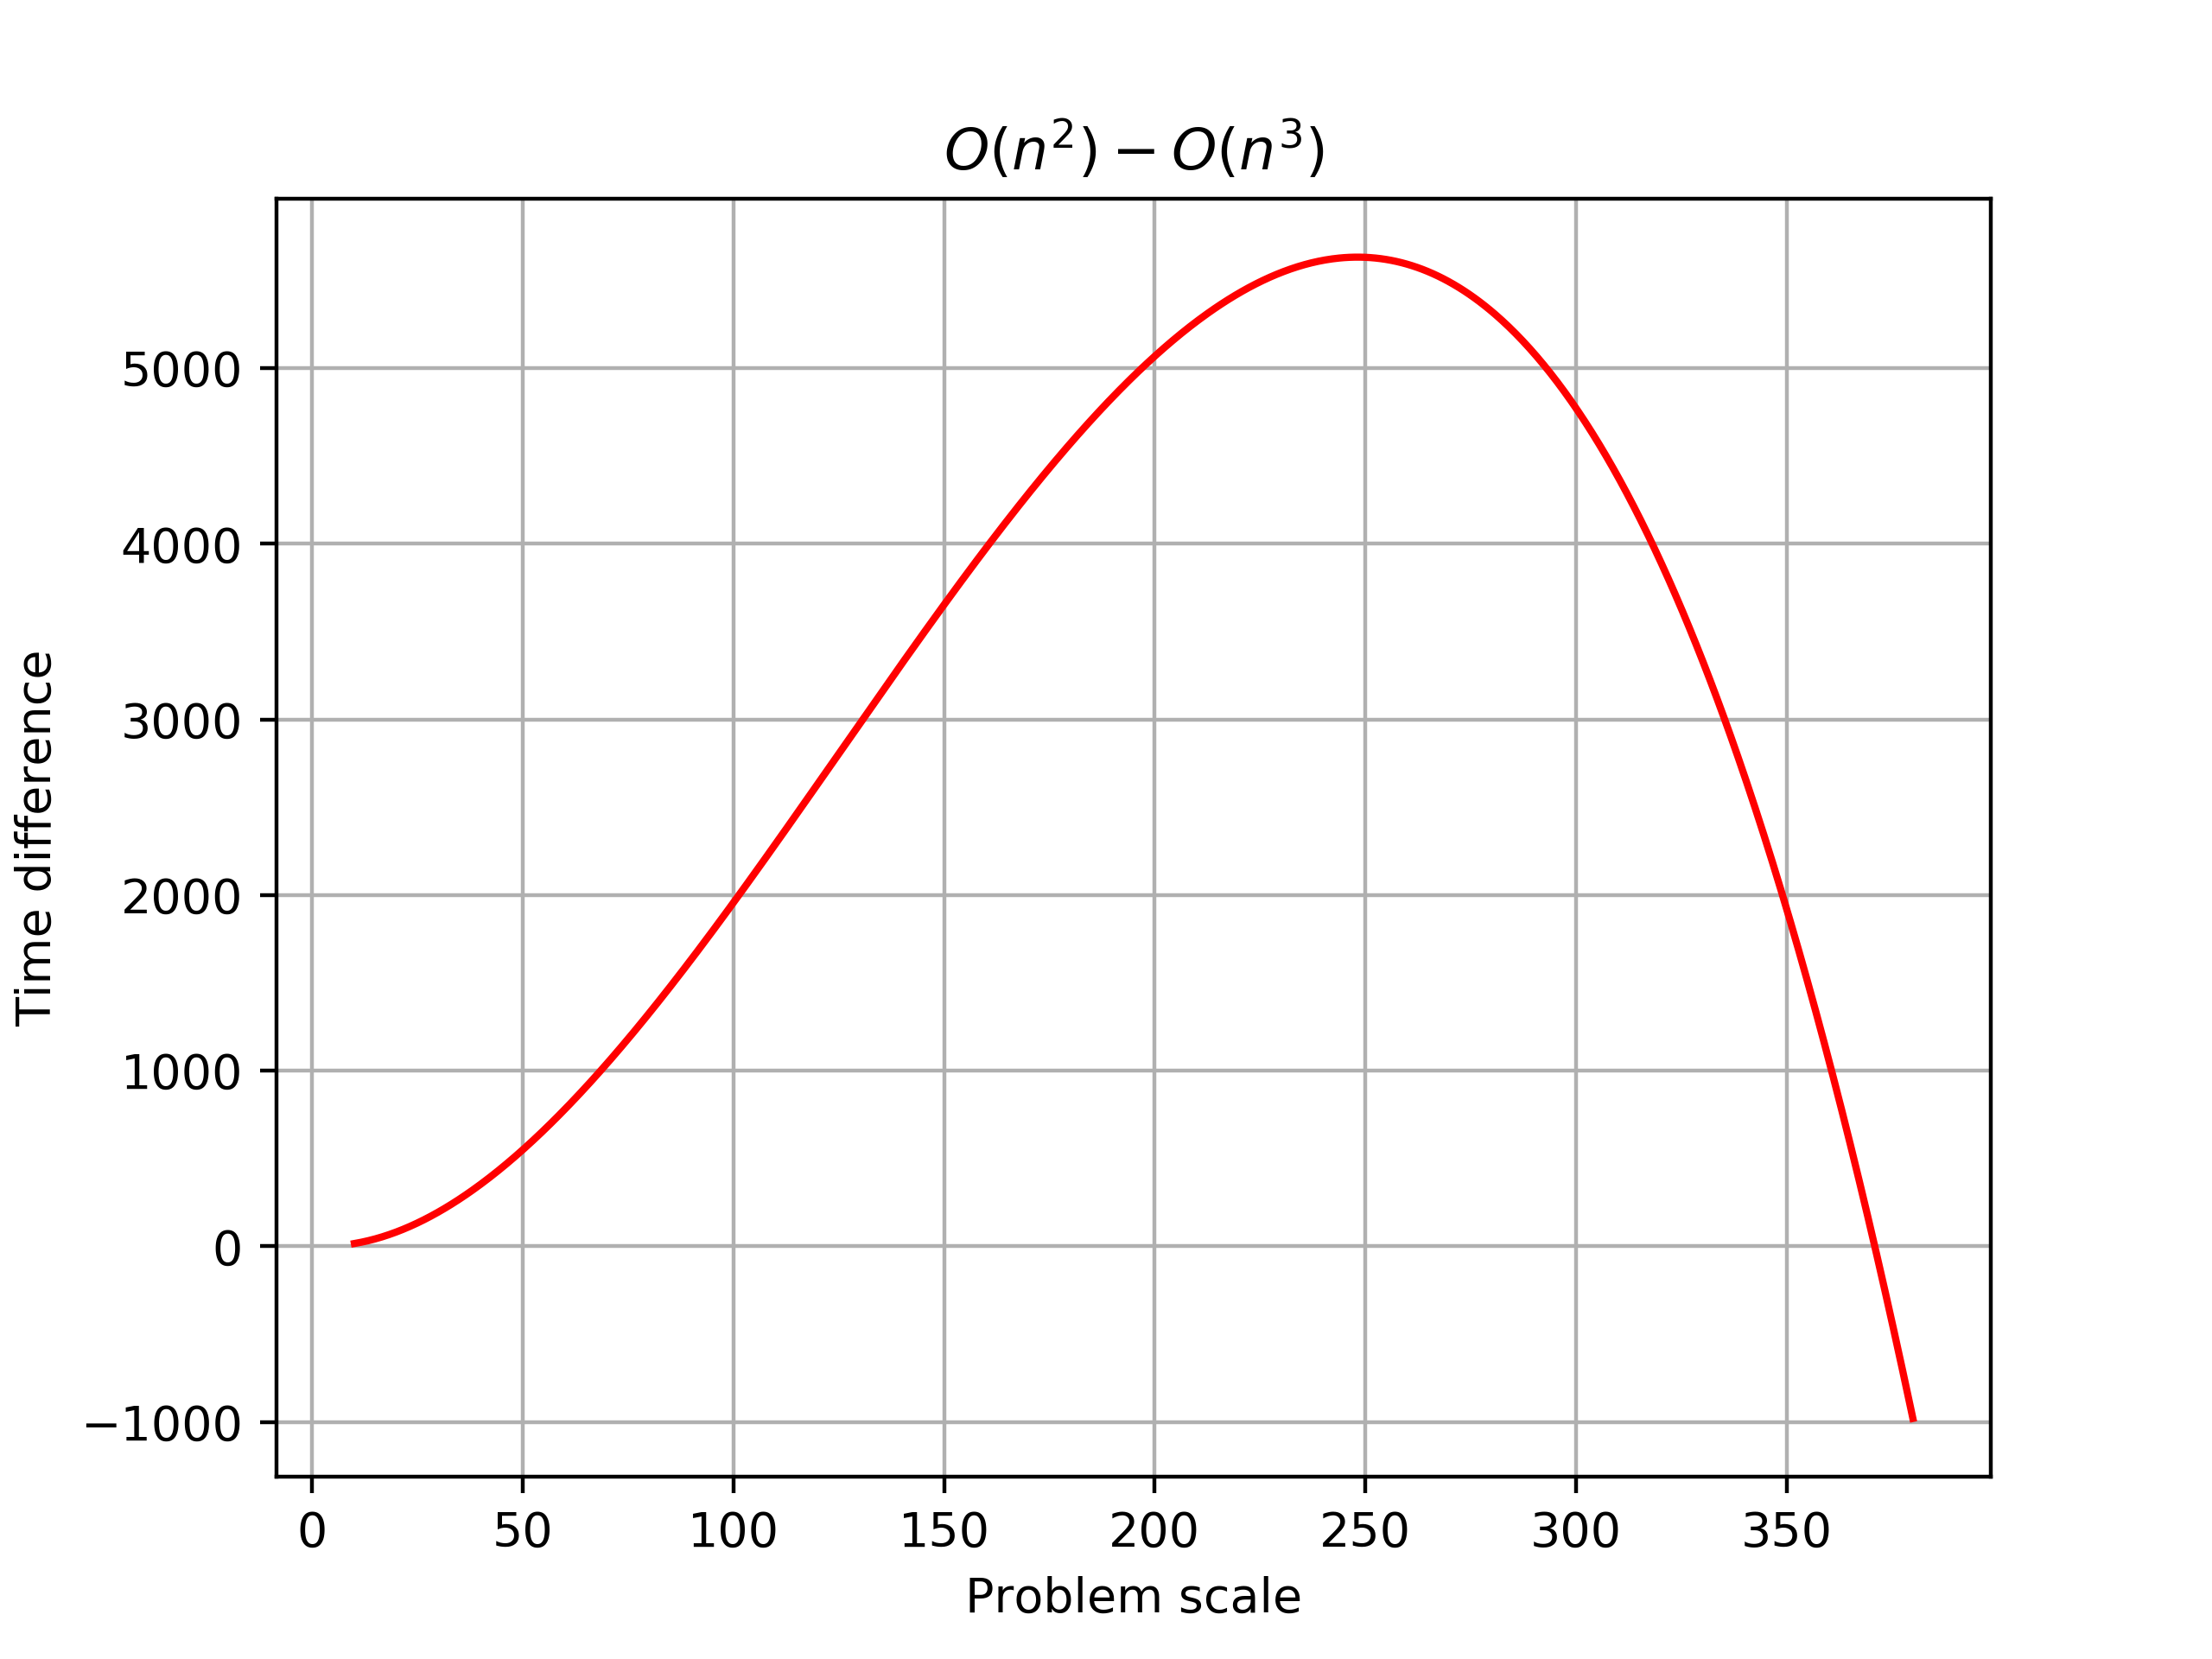
\includegraphics[scale=0.55]{figure/time-complexity.png}
            % \caption{算法时间复杂度的对比}
        \end{figure}
    \end{frame}

    \section{发挥设备优势}

    \begin{frame}{发挥设备优势}
        一个耗时1153秒的单进程任务:
        \begin{figure}[h]
            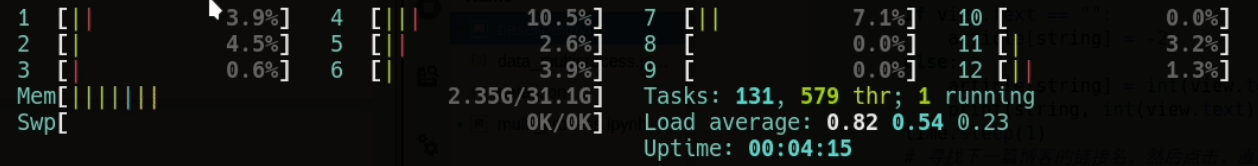
\includegraphics[scale=0.3]{figure/single.png}
            % \caption{单进程执行下的资源利用率}
        \end{figure}
        
        使用多进程改进,相同任务耗时105秒,且多核利用率较为均衡:
        \begin{figure}[h]
            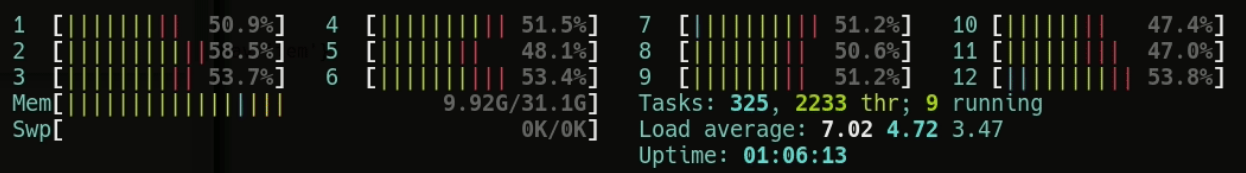
\includegraphics[scale=0.3]{figure/multi.png}
            % \caption{多进程执行下的资源利用率}
        \end{figure}
        
        \begin{leftbar}
        任务必须可以并行化。代码地址:{\sffamily \url{https://muyuuuu.github.io/2020/03/18/multi-process/}}
        \end{leftbar}
        
    \end{frame}

    \section{硬件与软件依赖}

    \begin{frame}{硬件与软件}
        \metroset{block=fill}
        \begin{exampleblock}{硬件部分}
            \begin{description}
                \item[{\ttfamily CPU}] 2个Intel(R) Xeon(R) Gold 5115 CPU \@ 2.40GHz,10核心20线程
                \item[{\ttfamily GPU}] 4路Tesla P40,每路显存容量22GB
                \item[内存] 128GB
                \item[外存] 520TB可用,已用15TB
            \end{description}
        \end{exampleblock}
        \metroset{block=fill}
        \begin{exampleblock}{软件部分}
            \begin{description}
                \item[系统] CentOS Linux release 7.3.1611 (执行), Arch 5.9.6(开发)
                \item[{\ttfamily python}] 3.8.2,开发语言
                \item[{\ttfamily pytorch}] 1.6.0,模型实现,借助其提供的API实现并行
                \item[{\ttfamily ssh}] OpenSSH\_8.3p1, OpenSSL 1.1.1h:实现远程登录
                \item[{\ttfamily scp}] 文件传输
            \end{description}
        \end{exampleblock}
    \end{frame}

    \begin{frame}{常用命令}
        \begin{alertblock}{命令行内执行}
            \begin{enumerate}
                \item {\ttfamily mv, cd, ls, cp, cat} 等文件操作
                \item {\ttfamily nohup python train.py > log} 挂起运行与重定向输出
                \item {\ttfamily ps -f|grep python} 查看挂起程序是否执行
            \end{enumerate}
        \end{alertblock}
    \end{frame}

    \section{模型}

    \begin{frame}{模型结构}
        \begin{leftbar}            
            实现的模型为Relation Network\footnote{\sffamily{\url{https://ieeexplore.ieee.org/abstract/document/8778601}}}。
            数据集为miniImageNet\footnote{\sffamily{\url{https://drive.google.com/file/d/0B3Irx3uQNoBMQ1FlNXJsZUdYWEE/view}}}。
        \end{leftbar}
        \begin{figure}[h]
            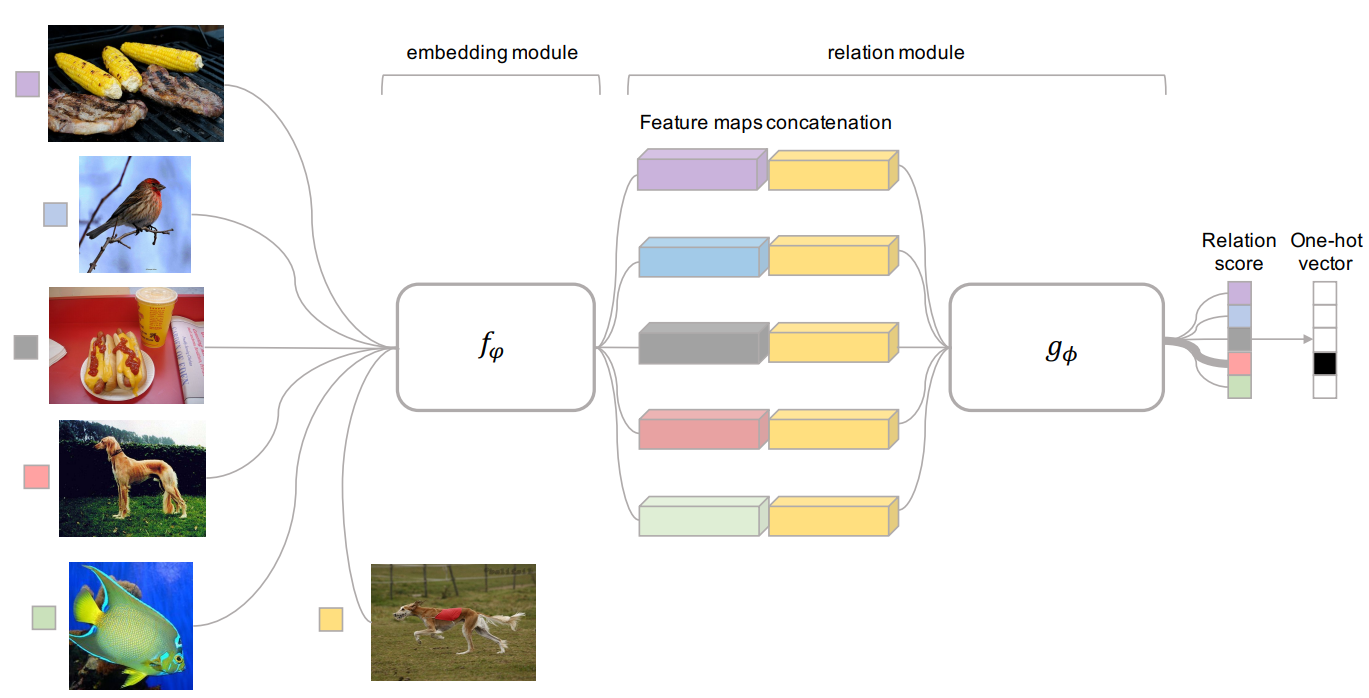
\includegraphics[scale=0.24]{figure/compare.png}
            % \caption{Relation Network结构图}
            % \label{fig:compare}
        \end{figure}
    \end{frame}



    \section{实验结果}
    
    \begin{frame}{DataParallel 单机多卡}
        \begin{leftbar}
            {\ttfamily nvidia-smi}查看显卡利用率:
        \end{leftbar}
        \begin{figure}
            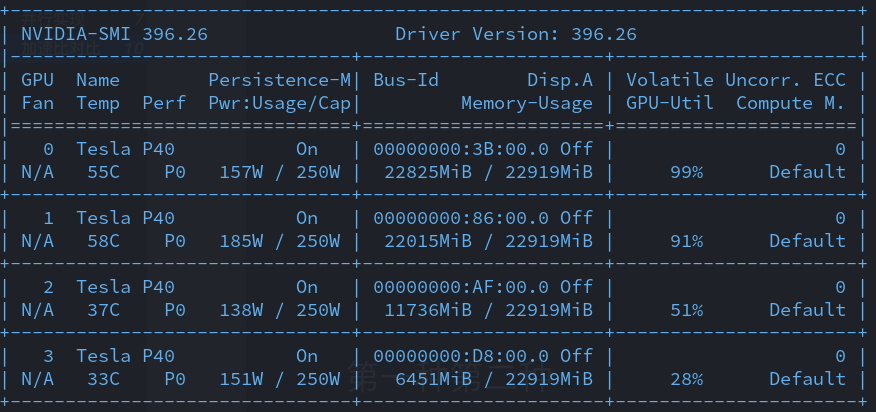
\includegraphics[scale=0.4]{figure/01gpu-use.png}
        \end{figure}
        程序执行时间:$T_1=137172$秒,约2286分钟,约1.59天。
    \end{frame}

    \begin{frame}{DistributedDataParallel 单机多卡}
        \begin{leftbar}
            {\ttfamily nvidia-smi}查看显卡利用率:
        \end{leftbar}
        \begin{figure}
            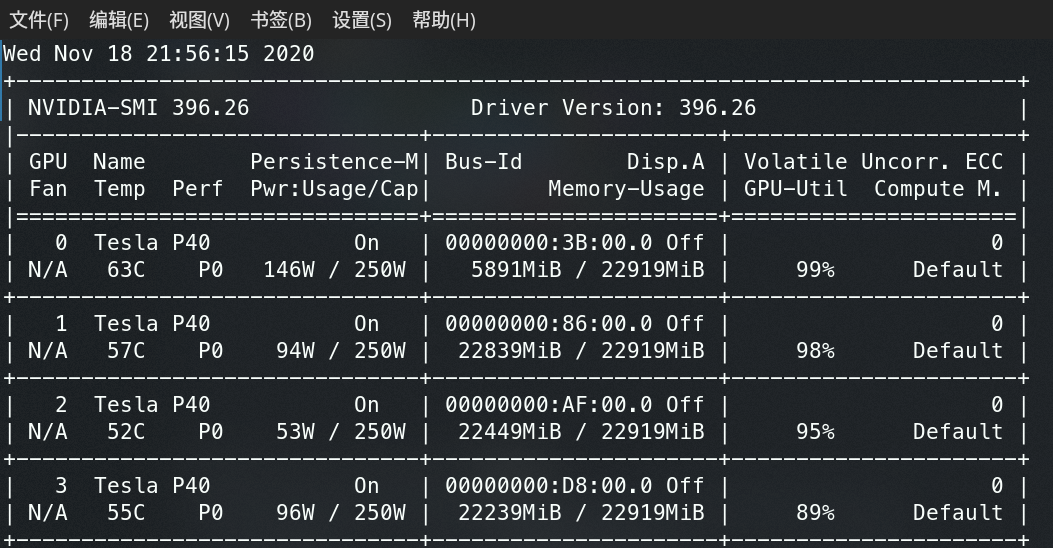
\includegraphics[scale=0.45]{figure/ddp.png}
        \end{figure}
        程序执行时间:$T_2=89856$秒,约1498分钟,约1.03天。
    \end{frame}

    \begin{frame}{DistributedDataParallel 单机多卡}
        \begin{leftbar}
            加速比:$\frac{T_1}{T_2}=1.53$
        \end{leftbar}
        \begin{leftbar}
            准确率对比:Dataparallel:0.566, DDP:0.582。
        \end{leftbar}
        \begin{leftbar}
            代码开放于:{\ttfamily \url{https://github.com/muyuuuu/Algorithm/tree/master/meta-learning/Metric-based/Relation-Netowrk}}
        \end{leftbar}
    \end{frame}


    % \begin{frame}
    %     \begin{columns}[T,onlytextwidth]
    %         \column{0.33\textwidth}
    %         \begin{block}{普通标题}
    %             \begin{itemize}
    %                 \item 普通内容
    %                 \item 普通内容
    %                 \item 普通内容
    %             \end{itemize}
    %         \end{block}
            % \metroset{block=fill}
            % \begin{block}{普通标题}
            %     \begin{itemize}
            %         \item 普通内容
            %         \item 普通内容
            %         \item 普通内容
            %     \end{itemize}
            % \end{block}
    %         \column{0.33\textwidth}
    %         \begin{alertblock}{警告标题}
    %             \begin{enumerate}
    %                 \item 警告内容
    %                 \item 警告内容
    %                 \item 警告内容
    %             \end{enumerate}
    %         \end{alertblock}
    %         \metroset{block=fill}
    %         \begin{alertblock}{警告标题}
    %             \begin{enumerate}
    %                 \item 警告内容
    %                 \item 警告内容
    %                 \item 警告内容
    %             \end{enumerate}
    %         \end{alertblock}
    %         \column{0.33\textwidth}
    %         \begin{exampleblock}{例子标题}
    %             \begin{description}
    %                 \item[描述定义] 描述内容
    %                 \item[描述定义] 描述内容
    %                 \item[描述定义] 描述内容
    %             \end{description}
    %         \end{exampleblock}
    %         \metroset{block=fill}
    %         \begin{exampleblock}{例子标题}
    %             \begin{description}
    %                 \item[描述定义] 描述内容
    %                 \item[描述定义] 描述内容
    %                 \item[描述定义] 描述内容
    %             \end{description}
    %         \end{exampleblock}
    %     \end{columns}
    % \end{frame}

    % \begin{fragile}
    %     \bicolumns{
    %         \begin{block}{图片}
    %             \begin{center}
    %                 % \includegraphics[width=0.65\textwidth]{cuzlogo}\\
    %                 % \includegraphics[width=0.65\textwidth]{cuzlogo-dark}\\
    %                 % \includegraphics[width=0.65\textwidth]{cuzlogo-light}\\
    %                 % \includegraphics[width=0.65\textwidth]{cuzlogo-brown}\\
    %             \end{center}
    %         \end{block}
    %     }{
    %     \begin{block}{表格}
    %         \begin{table}\small
    %             \begin{tabular}{llr}
    %                 \toprule
    %                 \multicolumn{2}{c}{项目} & \multirow{2}{*}{价格 (\$)} \\
    %                 \cmidrule(r){1-2}
    %                 动物                    & 描述 &  \\
    %                 \midrule
    %                 \multirow{2}{*}{蚋蚊}   & 每克 & 13.65 \\
    %                                         & 每只 & 0.01 \\
    %                 角马                    & 标本 & 92.50 \\
    %                 鸸鹋                    & 标本 & 33.33 \\
    %                 犰狳                    & 冷冻 & 8.99 \\
    %                 \bottomrule
    %             \end{tabular}
    %         \end{table}
    %     \end{block}
    %     }
    % \end{fragile}

    % \begin{fragile}[]
    %     \bicolumns[0.382]{
    %     }{
    %         \begin{block}{代码}
    %             \begin{minted}{c++}
    %                 // 西加加
    %                 #include <iostream>

    %                 auto main(int argc, char const **argv) {
    %                     std::cout << "Test" << std::endl;
    %                     return 0;
    %                 }
    %             \end{minted}
    %             \begin{minted}{java}
    %                 // 爪哇
    %                 public class Test {
    %                     public static void main(String[] args) {
    %                         System.out.println("Test");
    %                     }
    %                 }
    %             \end{minted}
    %             \begin{minted}{python}
    %     if device_ids is None:
    %         device_ids = _get_all_device_indices()

    %     if output_device is None:
    %         output_device = device_ids[0]
    %             \end{minted}
    %         \end{block}
    %     }
    % \end{fragile}

    % \begin{fragile}[]
    %     \bicolumns[0.382]{
    %     }{
    %         \begin{block}{算法}
    %             \begin{algorithmx}[alg:euclid]{Euclid算法}
    %                 \Procedure{Euclid}{$a,b$}\Comment{$a$与$b$的最大公约数}
    %                 \State $r\gets a\bmod b$
    %                 \While{$r\neq 0$}\Comment{若$r$为0则可跳出循环返回答案}
    %                 \State $a\gets b$
    %                 \State $b\gets r$
    %                 \State $r\gets a\bmod b$
    %                 \EndWhile\label{euclidendwhile}
    %                 \State \textbf{return} $b$\Comment{最大公约数为$b$}
    %                 \EndProcedure
    %             \end{algorithmx}
    %         \end{block}
    %     }
    % \end{fragile}

    \begin{standout}[]
        感谢聆听!
    \end{standout}

\end{document} 